\documentclass[crop,tikz, border=10pt]{standalone}% 'crop' is the default for v1.0, before it was 'preview'
\usepackage[compat=1.1.0]{tikz-feynman}
\begin{document}
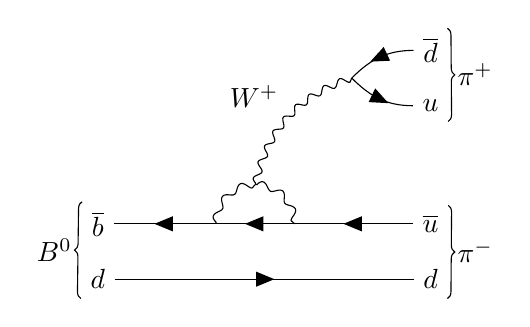
\begin{tikzpicture}
\begin{feynman}
\vertex (a1) {\(\overline b\)};
\vertex[right=1.5cm of a1] (a2);
\vertex[right=1cm of a2] (a3);
\vertex[right=1.5cm of a3] (a4) {\(\overline u\)};
\vertex[below=2em of a1] (b1) {\(d\)};
\vertex[below=2em of a4] (b2) {\(d\)};
%% See section 13.5 of PGF/TikZ manual
\vertex at ($(a2)!0.5!(a3)!0.5cm!90:(a3)$) (d);
%% Equivalent way to obtain (d):
% \vertex at ($(b2)!0.5!(b3) + (0, -0.5cm)$) (d);
\vertex[above=of a4] (c1) {\(u\)};
\vertex[above=2em of c1] (c3) {\(\overline d\)};
\vertex at ($(c1)!0.5!(c3) - (1cm, 0)$) (c2);
\diagram* {
(a4) -- [fermion] (a3) -- [fermion] (a2) -- [fermion] (a1),
(b1) -- [fermion] (b2),
(c3) -- [fermion, out=180, in=45] (c2) -- [fermion, out=-45, in=180] (c1),
(a2) -- [boson, quarter left] (d) -- [boson, quarter left] (a3),
(d) -- [boson, bend left, edge label=\(W^{+}\)] (c2),
};
\draw [decoration={brace}, decorate] (b1.south west) -- (a1.north west)
node [pos=0.5, left] {\(B^{0}\)};
\draw [decoration={brace}, decorate] (c3.north east) -- (c1.south east)
node [pos=0.5, right] {\(\pi^{+}\)};
\draw [decoration={brace}, decorate] (a4.north east) -- (b2.south east)
node [pos=0.5, right] {\(\pi^{-}\)};
\end{feynman}
\end{tikzpicture}

\end{document}
